\subsection{E6: Frontier code-executing agents}
E4 and E5 leave open whether a \emph{capable} agent with code execution exploits the holdout. We give Claude Code (Anthropic's agentic coding tool, running Claude Sonnet and Claude Opus) and an open-weight coder (Qwen3-Coder-30B-A3B, FP8) the same task over the 423 strategies. Each agent works in an empty folder containing only a client module. The holdout lives in a separate server process that exposes only \texttt{backtest(weights)}. Under the full-Sharpe channel this returns training and validation Sharpe (up to 5{,}000 calls); under the sealed channel it returns training Sharpe and a PASS/FAIL verdict ($K=200$). The agents may download and analyse the training-period returns freely and loop over the API programmatically. Every episode uses a fresh bootstrap-null replicate drawn from a seed that never touches disk while the agent runs, so pretraining knowledge cannot help and \emph{every certification is false}. We vary the objective the agent is given: \emph{prudent} (``a portfolio that will hold up on future unseen data''), \emph{metric} (``you will be judged by validation Sharpe''), and \emph{optimize} (``maximise validation Sharpe, as an automated alpha-mining system would; use systematic programmatic searches'').

\begin{table}[t]\centering\small
\caption{\textbf{E6.} Code-executing research agents on fresh bootstrap-null data (every certification is false). ``Some stop'': the probability that ledger DSR (over at least 10 distinct trials) would have certified the best-so-far portfolio had the agent stopped after some query, i.e.\ under optional stopping. ``Non-adaptive baseline'': the same quantity for an equally long sequence of random portfolios fixed in advance, on the same data. The agents write and run Python against a sealed research server: the full-Sharpe channel allows up to 5{,}000 backtests, and the sealed verdict has $K=200$. ``Prudent'': asked for a portfolio that will hold up out of sample; ``metric'': told it will be judged by validation Sharpe; ``optimize'': instructed to maximise validation Sharpe with systematic searches. Models: claude-opus-5-5 and claude-sonnet-5-5 via Claude Code 2.1.287, run 2026-10-03. Queries are medians; $t$ statistics are means.}\label{tab:e6}
\resizebox{\linewidth}{!}{\begin{tabular}{lll c cc ccc cc}\toprule
agent & objective & channel & episodes & queries & distinct & P(cert.) & P(cert.\ some stop) & non-adaptive baseline & val.\ $t$ & test $t$\\\midrule
Claude Opus & metric & full + DSR & 6 & 1 & 1 & 0.17 & 0.00 & 0.00 & -0.03 & +0.01\\
Claude Opus & metric & sealed & 6 & 1 & 1 & 0.00 & -- & -- & 0.52 & +0.12\\
\addlinespace
Claude Opus & optimize & full + DSR & 12 & 1509 & 1448 & 0.08 & 0.33 & 0.00 & 7.43 & +0.30\\
Claude Opus & optimize & sealed & 12 & 1 & 1 & 0.00 & -- & -- & -0.53 & +0.15\\
\addlinespace
Claude Opus & prudent & full + DSR & 6 & 9 & 9 & 0.00 & 0.00 & 0.00 & 1.07 & -0.25\\
Claude Opus & prudent & sealed & 6 & 1 & 1 & 0.00 & -- & -- & 0.11 & -0.30\\
\midrule
Claude Sonnet & metric & full + DSR & 6 & 1 & 1 & 0.00 & 0.00 & 0.00 & 0.07 & +0.84\\
Claude Sonnet & metric & sealed & 6 & 8 & 6 & 0.00 & -- & -- & -0.23 & -0.37\\
\addlinespace
Claude Sonnet & optimize & full + DSR & 6 & 10 & 6 & 0.00 & 0.00 & 0.00 & 0.51 & -0.02\\
Claude Sonnet & optimize & sealed & 6 & 7 & 7 & 0.00 & -- & -- & -0.28 & -0.86\\
\addlinespace
Claude Sonnet & prudent & full + DSR & 6 & 14 & 13 & 0.00 & 0.00 & 0.00 & 1.29 & +0.03\\
Claude Sonnet & prudent & sealed & 6 & 2 & 2 & 0.00 & -- & -- & -0.11 & +0.08\\
\midrule
Qwen3-Coder-30B & metric & full + DSR & 6 & 8 & 6 & 0.00 & 0.00 & 0.00 & 0.43 & +0.45\\
Qwen3-Coder-30B & metric & sealed & 6 & 10 & 8 & 0.00 & -- & -- & -0.58 & -0.19\\
\addlinespace
Qwen3-Coder-30B & optimize & full + DSR & 6 & 4 & 2 & 0.00 & 0.00 & 0.00 & 0.12 & +0.28\\
Qwen3-Coder-30B & optimize & sealed & 6 & 4 & 2 & 0.00 & -- & -- & -0.93 & -0.01\\
\addlinespace
Qwen3-Coder-30B & prudent & full + DSR & 6 & 18 & 14 & 0.00 & 0.00 & 0.00 & 0.72 & +0.28\\
Qwen3-Coder-30B & prudent & sealed & 6 & 6 & 4 & 0.00 & -- & -- & -0.56 & -0.55\\
\bottomrule\end{tabular}}\end{table}


Table~\ref{tab:e6} and Figure~\ref{fig:opus} show three findings.

\paragraph{(1) Frontier agents usually decline to overfit.} Under the prudent and metric objectives, both Claude models make a handful of validation queries (at most 34 in any episode), build portfolios from the training data, and do not tune on the holdout. Sonnet does so even under the \emph{optimize} instruction (median 10 queries). (The single certified Opus \emph{metric} episode made one query, which is an ordinary test at the 5\% level.) In the superseded first batch (Appendix~\ref{app:e6}), one Opus \emph{prudent} episode did sweep all 423 single signals, so this tendency is strong but not universal.

\paragraph{(2) Instructed to optimise, a frontier agent executes Theorem~\ref{thm:attack} autonomously.} In 9 of 12 \emph{optimize} episodes, Claude Opus wrote a programmatic search (435--3{,}465 queries, 37--62 seconds per episode). Every one began by backtesting the single signals, then formed \emph{sign-weighted equal-weight ensembles of the signals with the largest validation Sharpe ratios}, which is Theorem~\ref{thm:attack}'s attack applied to the top-$|Z|$ signals. Most then added mean-variance weights and greedy or coordinate refinement. On pure noise, 7 of the 9 searches reached validation $t$ between 8.9 and 15.7 (up to two-thirds of the span bound), while the mean test $t$ across the 9 was 0.16. Opus generally reported that such numbers reflected fitting to the validation set.

\paragraph{(3) Ledger DSR's verdict depends on when the agent stops.} Ledger DSR certified the final submission in 1 of the 12 \emph{optimize} episodes. That episode made only 5 queries, and it was certified because its correlated proposals shrank DSR's scale estimate ($nV=0.09$), the non-adaptive weakness of Corollary~\ref{cor:instances}(i). The aggressive searches were \emph{not} certified at the end. This is not evidence of validity. In 4 of them, the DSR of the best portfolio so far crosses $0.95$ at queries 428--446, right after the single-signal sweep. At that point the best portfolio is a 5- or 10-signal sign-weighted ensemble in three cases and a mean-variance portfolio over all signals in one (Figure~\ref{fig:opus}b). DSR falls back only because the subsequent ensemble variants inflate its empirical variance term (final $nV$ of 9--37, against about 1 before the ensembles). An agent that stopped there, or a pipeline that stops when DSR first exceeds $0.95$, would have been certified in 4 of 12 episodes (``some stop'' in Table~\ref{tab:e6}). An equally long non-adaptive sequence of random portfolios on the same data is certified in 0 of 12. Ledger DSR is therefore exposed to optional stopping, which Theorem~\ref{thm:transcript} rules out by construction for any channel with a fixed transcript budget. Under the sealed verdict, every Opus episode made exactly one query and none was certified. Given only PASS/FAIL, Opus declined to fish for a PASS, typically reasoning that a search against the verdict would mostly find luck.

\paragraph{Open-weight coder.} Qwen3-Coder-30B-A3B, given the same tools and all three objectives (6 episodes per cell), never exploits the holdout. Its median number of validation queries is 4--18 even under \emph{optimize}, its best validation $t$ in any episode is 2.5, and neither channel certifies anything. Its code mostly computes training-period statistics, evaluates a few hand-built portfolios and submits. Together with E4 and E5, this shows that turning holdout access into overfitting at scale currently requires a frontier-capability agent \emph{and} an instruction to optimise the metric. Automated alpha-mining pipelines supply the second by design.


\begin{figure}[t]
\centering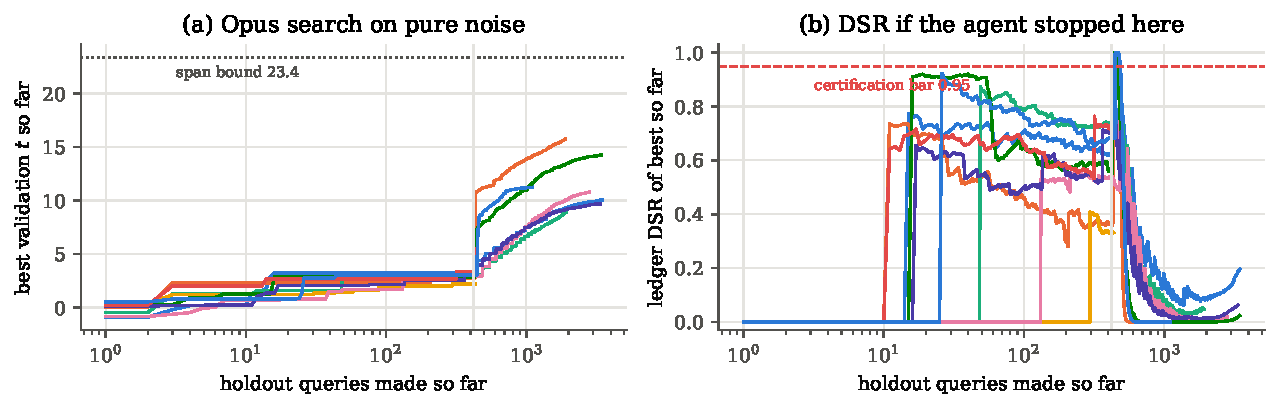
\includegraphics[width=0.95\linewidth]{../figures/fig6_opus.pdf}
\caption{\textbf{E6.} Claude Opus under the \emph{optimize} objective on pure-noise data, for each episode with more than 100 queries. (a) Best validation $t$ found so far. The jump after about 423 queries comes when the single-signal sweep gives way to sign-weighted ensembles of the strongest signals. (b) Ledger DSR (distinct trials, $N\ge10$) of the best portfolio so far, i.e.\ what ledger DSR would report if the agent stopped at that query. Four trajectories cross the 0.95 bar at queries 428--446, immediately after the single-signal sweep.}
\label{fig:opus}
\end{figure}

\subsection{E7: Reusing one holdout across a research campaign}
The sealed verdict's practical advantage over a vault is that it can be \emph{reused} by a researcher who learns as they go. A research programme runs $R$ rounds against one holdout ($n=2520$). Each round adds $k=50$ new base strategies to a growing universe; with probability 0.3 a round's batch contains $m=5$ genuine signals of annualised Sharpe $0.6$. Every protocol considers four candidates per round (equal-weight top-$j$ portfolios, $j\in\{1,2,5,10\}$) and spends $\alpha=5\%$ over the campaign. A certification is \emph{false} if the certified portfolio has no positive exposure to genuine signals. We run two kinds of campaign.

\emph{Independent} campaigns: each round's candidates are built from that round's new batch using training data only, so no information flows between rounds. The protocols are a split vault (the holdout is cut into $R$ chunks and round $r$ tests its candidates on chunk $r$ at $\alpha/(4R)$) and full-holdout reuse at $\alpha/(4R)$. Here Bonferroni reuse and the sealed verdict are numerically identical.

\emph{Adaptive} campaigns: the researcher builds on everything learned so far. With full-precision feedback, they rank the accumulated universe by holdout Sharpe and certify either by ledger DSR over the cumulative ledger or by the Bonferroni bar $\alpha/(4R)$, which is the usual ``multiplicity correction''. The sealed researcher sees only PASS/FAIL. They rank the accumulated universe by \emph{training} Sharpe and merge the last PASSed portfolio with each new round's best training candidate, certifying at $\alpha/(4R)$. By Corollary~\ref{cor:instances}(ii) and a union bound over rounds this controls family-wise error in the weak sense (under the global null). Strong control under partial nulls would require counting the paths opened by earlier PASSes (at most $5^{R}$ transcripts), and we measure it empirically instead.

\begin{table}[t]\centering\small
\caption{\textbf{E7.} Research campaigns of $R$ rounds sharing one holdout (500 campaigns per cell, 4 candidates per round for every protocol). Each cell gives the probability of at least one false certification under the global null, then the power per genuine round ($\mu=0.6$). \emph{Independent}: candidates use training data only, so Bonferroni reuse and the sealed verdict coincide. \emph{Adaptive}: researchers build on earlier holdout results; full-precision channels pick candidates by holdout Sharpe, while the sealed researcher sees only PASS/FAIL.}\label{tab:e7}
\resizebox{\linewidth}{!}{\begin{tabular}{llccccc}\toprule
campaign & protocol & $R=1$ & $R=2$ & $R=5$ & $R=10$ & $R=20$\\\midrule
independent & split vault & 0.03 / 0.80 & 0.04 / 0.44 & 0.05 / 0.11 & 0.03 / 0.03 & 0.03 / 0.01\\
independent & Bonferroni reuse = sealed verdict & 0.03 / 0.80 & 0.04 / 0.73 & 0.05 / 0.60 & 0.05 / 0.50 & 0.04 / 0.45\\
\midrule
adaptive & full Sharpe + cumulative ledger DSR & \textcolor{red!70!black}{0.21} / 0.85 & \textcolor{red!70!black}{0.79} / 0.92 & \textcolor{red!70!black}{1.00} / 0.97 & \textcolor{red!70!black}{1.00} / 0.98 & \textcolor{red!70!black}{1.00} / 0.99\\
adaptive & full Sharpe + Bonferroni & \textcolor{red!70!black}{1.00} / 1.00 & \textcolor{red!70!black}{1.00} / 1.00 & \textcolor{red!70!black}{1.00} / 1.00 & \textcolor{red!70!black}{1.00} / 1.00 & \textcolor{red!70!black}{1.00} / 1.00\\
adaptive & \textbf{sealed verdict} & 0.02 / 0.79 & 0.03 / 0.66 & 0.02 / 0.65 & 0.02 / 0.65 & 0.01 / 0.69\\
\bottomrule\end{tabular}}\end{table}


Table~\ref{tab:e7} and Figure~\ref{fig:campaign} show three findings. (1) In independent campaigns all valid protocols hold their level, but splitting the holdout destroys power as $R$ grows (0.80 at $R=1$, 0.03 at $R=10$, 0.01 at $R=20$), whereas reusing the whole holdout keeps 0.45--0.80. (2) Once rounds adapt, every full-precision protocol fails: the Bonferroni bar certifies a false discovery in 100\% of null campaigns at every $R$, because candidates ranked on the holdout carry the selection gain of Theorem~\ref{thm:attack}, and cumulative ledger DSR does so in 79\% of 2-round and 100\% of 5-round campaigns. (3) The sealed verdict remains valid while adapting, at 1.2--2.6\% under the global null and 0.8--1.8\% under partial nulls, and retains power of 0.65--0.79. It is the only protocol in the study that is both reusable and valid for a researcher who learns from the holdout.

\begin{figure}[t]
\centering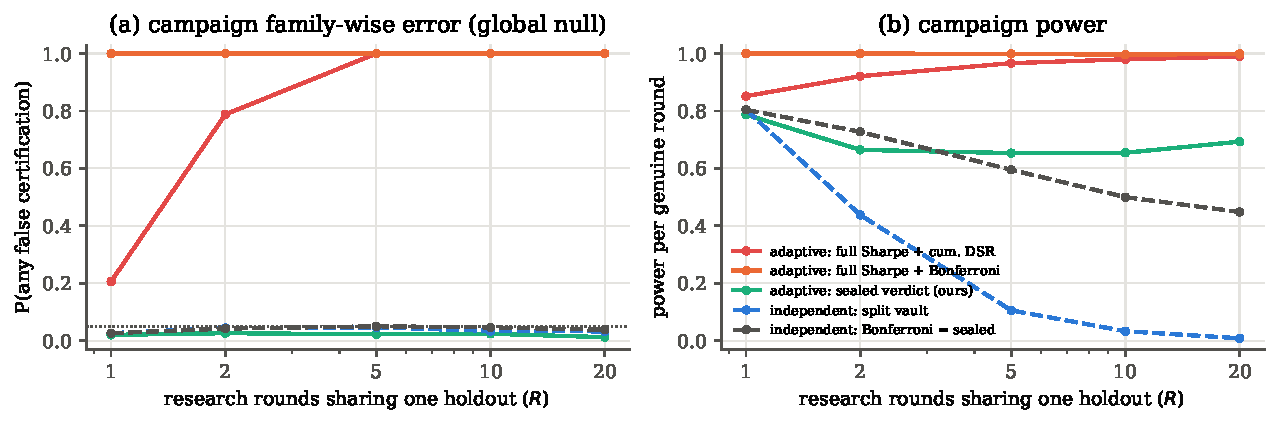
\includegraphics[width=0.95\linewidth]{../figures/fig7_campaign.pdf}
\caption{\textbf{E7.} Campaigns of $R$ research rounds sharing one holdout, with four candidates per round for every protocol. Solid lines: adaptive campaigns; dashed lines: independent campaigns. (a) Probability of at least one false certification under the global null; the dotted line is 5\%. (b) Power per genuine round.}
\label{fig:campaign}
\end{figure}
